\section{Техническое задание на систему и её составляющие} \label{sect:task}

На Рисунке \ref{fig:SystemDraft} показана структурная схема типичной системы связи для IoT. IoT модуль собирает данные телеметрии и(ли) управляет какой-либо системой, для того чтобы обеспечить связь модуля с сетью сервером IoT и с сетью Интернет вообще, требуется базовая станция, которая будет преобразовывать и перенаправлять пакеты между сетями. 

\begin{figure}[H]
	\centering
	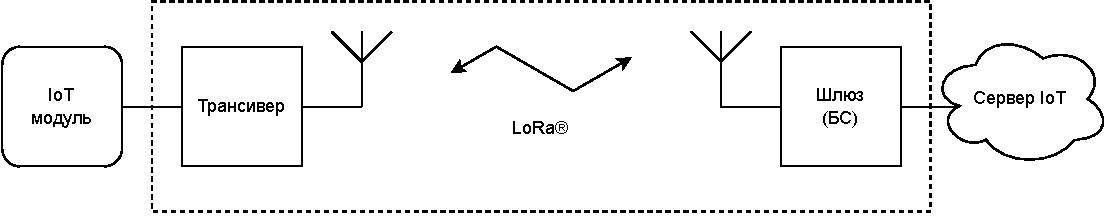
\includegraphics[width=0.9\textwidth,keepaspectratio]{SystemDraft.pdf}
	\caption{Структурная схема типичной системы связи для IoT}%
	\label{fig:SystemDraft}
\end{figure}

Необходимо разработать подсистему связи базовой станции (далее просто БС) и мобильное оконечное устройство (далее МОУ), использующие технологию LoRa. Для мобильного модуля также необходимо разработать компактную антенну. 

Все устройства системы должны удовлетворять стандарту RU864-870 и соответствовать требованиям, определяемых Приложением 11 к решению \linebreak ГКРЧ от 07.05.2007 №07-20-03-001:

\begin{longtblr}[
	caption = { Региональные стандарты, выдержка.},
	label = {table:regional-std}
	]{
		colspec={Q[223,l,m]Q[198,l,m]Q[429,l,m]},width=1.05\textwidth,
		vlines,hlines,
		vspan=even,
		rowhead=1,
		row{1}={font=\bfseries}
	}
	%%%%%%%%%%%%%%%%%%%%%%%%%%%%%%%%%%%%%%%%%%%%%%%
	Полоса радиочастот, МГц & Максимальная ЭИИМ, мВт &  Ограничения \\
	%%%%%%%%%%%%%%%%%%%%%%%%%%%%%%%%%%%%%%%%%%%%%%%%
	864 -- 865 		& 25 & Рабочий цикл 0,1\% или режим LBT \\
	868,7 -- 869,2 	& 25 & Рабочий цикл 0,1\% или режим LBT \\
\end{longtblr}

Средняя скорость передачи данных в сети должна быть не менее 1 кб/с

Основными требованиями к БС являются:
\begin{itemize}
	\setlength\itemsep{-1ex}
	\item Одновременная обработка данных от нескольких устройств
	\item Чувствительность не более минус 120 дБм
	\item Максимальная выходная мощность 12-14 дБм
\end{itemize}

Основными требованиями к МОУ являются:

\begin{itemize}
	\setlength\itemsep{-1ex}
	\item Возможность работы от аккумулятора или другого компактного источника питания
	\item Размеры (ДхШ) не более 6х6 см
	\item Чувствительность не более минус 120 дБмВт
	\item Максимальная выходная мощность 10-14 дБмВт
\end{itemize}

Основными требованиями к мобильной антенне являются всенаправленность и наибольший линейный размер в пределах 20 мм.


